\documentclass{ProblemSetCUNY}
\usepackage{bussproofs} \EnableBpAbbreviations
\usepackage{mathrsfs}
\usepackage{stix}
\usepackage{pgffor}
\usepackage{bm}
\usepackage{microtype}
\usepackage{nicematrix}

\usepackage{tikz}


\usepackage{tabstackengine}
\TABstackMath
\TABbinary

\AssignmentNumber{3}%
\CourseName{Probability and Statistics for Computer Science}
\CourseNumber{217}
\InstructorName{Alex Washburn}
\DueDateYear{2023}
\DueDateMonth{09}
\DueDateDay{18}


%\newenvironment{\ContactListing}[args]{begdef}{enddef}

\newcommand{\ProofLabelOne}[1]{\RightLabel{\ensuremath{\Parens{\mathrm{\textsc{#1}}}}\xspace}}
\newcommand{\ProofLabelTwo}[2]{\RightLabel{\ensuremath{\Parens{\mathrm{\textsc{#1}}}\Parens{\mathrm{#2}}}\xspace}}

\newcommand{\LogicCase}[1]{\item \textbf{Case}~#1:\newline}

\newcommand{\DerivationFormat}[2]{\hfill\qquad#2\textsc{#1}}
\newcommand{\Derivation}[2]{\DerivationFormat{#1}{#2~\ensuremath{\ruledelayed}~}}

\newcommand{\AxiomCL}[1]{\DerivationFormat{Axiom~#1}{}}
\newcommand{\Factivity}{\DerivationFormat{Factivity}{}}
\newcommand{\Given}{\DerivationFormat{Hypothesis}{}}
\newcommand{\Contrapositive}{\DerivationFormat{Contrapositive}{}}
\newcommand{\DoubleNegation}{\DerivationFormat{Double Negation}{}}
\newcommand{\DeMorgans}{\DerivationFormat{DeMorgans}{}}
\newcommand{\Necitation}[1]{\Derivation{Necitation}{#1}}
\newcommand{\Distribution}[1]{\Derivation{Distribution}{#1}}
\newcommand{\Reflexivity}[1]{\Derivation{Reflexivity}{#1}}
\newcommand{\ConDef}[1]{\Derivation{Connective Definition}{#1}}
\newcommand{\Contradiction}[1]{\ensuremath{\neg \phi \land \phi}\Derivation{Contradiction}{\ensuremath{\phi = #1}}}
\newcommand{\DedThm}[1]{\Derivation{Deduction Theorem}{#1}}
\newcommand{\ModPon}[2]{\Derivation{Modus Ponens}{#1, #2}}
\newcommand{\Syllogism}[2]{\Derivation{Syllogism}{#1, #2}}
\newcommand{\Theorem}[2]{\DerivationFormat{Theorem~--~Lecture~#1,~Page~#2}{}}

\newcommand{\?}{\stackrel{?}{=}}
\newcommand{\R}[2]{\ensuremath{\World{#1}\mathrel{R}\World{#2}}\xspace}
\newcommand{\Tr}[2]{\ensuremath{\tau\Parens{#1,\,#2}\xspace}}
\newcommand{\T}[1]{\ensuremath{\tau\Parens{#1}\xspace}}
\newcommand{\Prob}[1]{\ensuremath{P\Parens{#1}}\xspace}
\newcommand{\ProbGiven}[2]{\ensuremath{P\Parens{#1\,|\,#2}}\xspace}
\newcommand{\Event}[1]{\ensuremath{\bm{\mathsf{#1}}}\xspace}
\newcommand{\RandVar}[1]{\ensuremath{\mathbf{#1}}\xspace}
\newcommand{\DistMap}[2]{~#1&\mapsto~~#2\\}
\newcommand{\DistCondition}[2]{~#1&\text{\normalfont iff}~~#2\\}

\newcommand{\Hint}[1]{\textit{\textls{Hint:}~#1}}

\newcommand{\One}{\ensuremath{\textbf{1}}\xspace}

\newcommand{\Heads}{\ensuremath{\mathtt{H}}\xspace}
\newcommand{\Tails}{\ensuremath{\mathtt{T}}\xspace}

\newcommand{\Die}[1]{\ensuremath{\mathbf{D}_{#1}}\xspace}
\newcommand{\Above}[1]{\ensuremath{\overline{#1}}\xspace}
\newcommand{\Below}[1]{\ensuremath{\underline{#1}}\xspace}
\newcommand{\Num}[1]{\ensuremath{\mathbb{#1}}\xspace}
\newcommand{\NumA}[1]{\ensuremath{\overline{\Num{#1}}}\xspace}
\newcommand{\NumB}[1]{\ensuremath{\underline{\Num{#1}}}\xspace}

\newcommand{\EquivGrid}{\ensuremath{~\;\;\equiv\quad}\xspace}




\newcommand{\Countermodel}[4]{%
\textbf{Countermodel} $\mathcal{K}$ in #1:%
\begin{itemize}%
\item \ensuremath{W = \SetNote{\World{0}%
\foreach \n in {1,...,#2}{,~\World{\n}}%
}}%
\item \ensuremath{\mathrel{R}~=~#3}%
\item #4%
\end{itemize}%
}

\begin{document}
\CoverPage%

\newcommand{\Bullet}[3]{\hspace*{4mm}\ensuremath{\Parens{\Event{#1}}}:\hspace*{2mm}#2\[#3\]\\[5mm]}
\newcommand{\BulletLine}[3]{\hspace*{4mm}\ensuremath{\Parens{\Event{#1}}}:\hspace*{2mm}#2\hfill\ensuremath{#3}\\[5mm]}

\Problem{%
Alice and Bob each choose at random real-valued numbers $\RandVar{A}$ and $\RandVar{B}$ (respectively) from the continuous interval $\NumericRange{0}{3}$.
We assume a uniform probability law under which the probability of an event is proportional to its area.
Consider the following events:\\[5mm]
\Bullet{W}
{The magnitude of the difference of $\RandVar{A}$ and $\RandVar{B}$ is greater than $\frac{2}{3}$.}
{\left|\,\RandVar{A} - \RandVar{B}\,\right| > \frac{2}{3}}
\Bullet{X}
{At least one of the numbers is greater than $\frac{2}{3}$.}
{\RandVar{A} > \frac{2}{3}\;\lor\;\RandVar{B} > \frac{2}{3}}
\Bullet{Y}
{Alice’s number is greater than $\frac{2}{3}$.}
{\RandVar{A} > \frac{2}{3}}
\Bullet{Z}
{The two numbers are equal.}
{\RandVar{A} = \RandVar{B}}
\Hint{Draw the 2D space of $\NumericRange{0}{3} \times \NumericRange{0}{3}$ and shade the event areas.}
}


\SubProblem{Find the probability \Prob{\Event{W}}.}
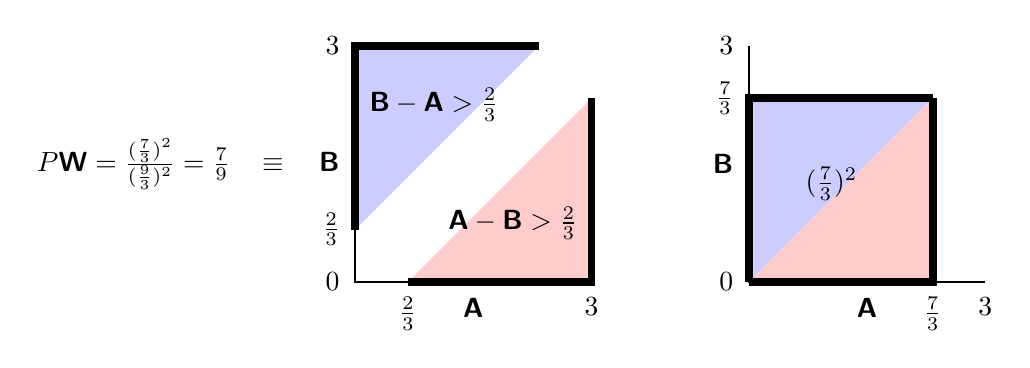
\begin{tikzpicture}
\draw[thick] (0,3) node[left=2pt] {$3$} -- node[left=2pt] {$\Prob{\Event{W}} = \frac{(\frac{7}{3})^2}{(\frac{9}{3})^2} = \frac{7}{9} \EquivGrid
\Event{B}$} (0,0)
 node[left=2pt] {$0$} -- node[below=2pt] {$\Event{A}$} (3,0) node[below=2pt] {$3$};
\draw[line width=1mm,fill=red!20] (0.667,0) -- (3,0) -- (3,2.333)  
 (2, 0.75) node{$\Event{A} - \Event{B} > \frac{2}{3}$};
\draw[line width=1mm,fill=blue!20] (0,0.667) -- (0,3) -- (2.333,3)
 (1, 2.25) node {$\Event{B} - \Event{A} > \frac{2}{3}$};
\draw (3.667, 1.5) node {$\rightsquigarrow$};
\draw[thick] (5,3) node[left=2pt] {$3$} -- node[left=2pt] {$
\Event{B}$} (5,0) 
 node[left=2pt] {$0$} -- node[below=2pt] {$\Event{A}$} (8,0) node[below=2pt] {$3$};
\draw[line width=1mm,fill=blue!20] (5,0) -- (5, 2.333) -- (7.333,2.333);
\draw[line width=1mm,fill=red!20] (5,0) -- (7.333,0) -- (7.333,2.333);
\node[left=2pt] at (0,0.667) {$\frac{2}{3}$};
\node[below=2pt] at (0.667,0) {$\frac{2}{3}$};
\node[left=2pt] at (5,2.333) {$\frac{7}{3}$};
\node[below=2pt] at (7.333,0) {$\frac{7}{3}$};
\node[left=0pt] at (6.5, 1.25) {$(\frac{7}{3})^2$};
 \end{tikzpicture}
 \[
 \Prob{\Event{W}} =  \frac{(\frac{7}{3})^2}{(\frac{9}{3})^2} = \frac{49}{81} \approx 0.605\\
 \]
 
 
\SubProblem{Find the probability \Prob{\Event{Z}}.}
\begin{tikzpicture}
\draw[thick] (0,3) node[left=2pt] {$3$} -- node[left=2pt] {$\Prob{\Event{Z}} =  \Prob{\RandVar{A} = \RandVar{B}} = 0 \EquivGrid
\Event{B}$} (0,0)
 node[left=2pt] {$0$} -- node[below=2pt] {$\Event{A}$} (3,0) node[below=2pt] {$3$};
\draw[line width=0mm] (0,0) -- (3,3);
 \end{tikzpicture}
\[
\Prob{\Event{Z}} =  \Prob{\RandVar{A} = \RandVar{B}} = 0\quad\text{Because the area of the line}~\RandVar{A} = \RandVar{B}~\text{has no area!}
\]

\SubProblem{Find the probability \ProbGiven{\Event{X}}{\Event{Y}}.}

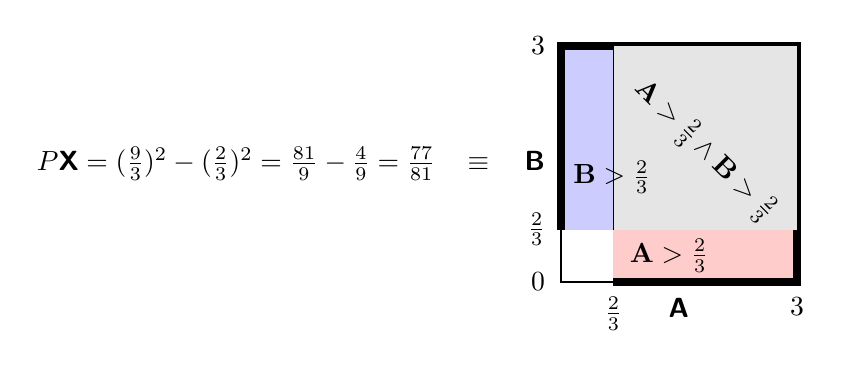
\begin{tikzpicture}
\draw[thick] (0,3) node[left=2pt] {$3$} -- node[left=2pt] {$\Prob{\Event{X}} = (\frac{9}{3})^2 - (\frac{2}{3})^2=  \frac{81}{9} - \frac{4}{9} = \frac{77}{81}\EquivGrid
\Event{B}$} (0,0)
 node[left=2pt] {$0$} -- node[below=2pt] {$\Event{A}$} (3,0) node[below=2pt] {$3$};
\draw[line width=1mm,fill=red!20] (0.667,0) -- (3,0) -- (3,3) -- (0.667,3);
\draw[line width=1mm,fill=blue!20] (0,0.667) -- (0,3) -- (3,3) -- (3,0.667);
\draw[line width=0mm,fill=gray!20] (3,0.667) -- (3,3) -- (0.667,3) -- (0.667,0.667);
\node[left=0pt] at (2, 0.333) {$\RandVar{A} > \frac{2}{3}$};
\node[right=1pt] at (0, 1.333) {$\RandVar{B} > \frac{2}{3}$};
\node[left=0pt,rotate=315] at (2.75, 0.75) {$\RandVar{A} > \frac{2}{3} \land\RandVar{B} > \frac{2}{3}$};
\node[left=2pt] at (0,0.667) {$\frac{2}{3}$};
\node[below=2pt] at (0.667,0) {$\frac{2}{3}$};
 \end{tikzpicture}

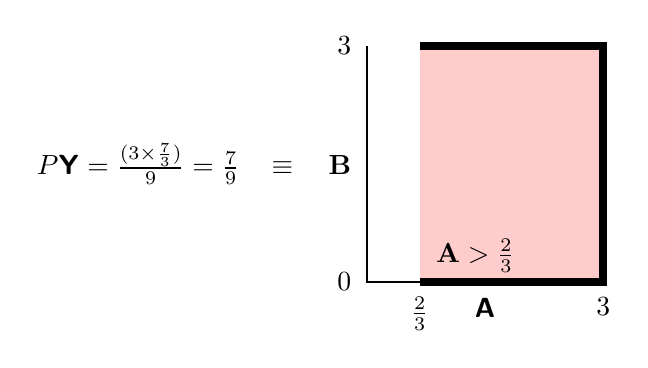
\begin{tikzpicture}
\draw[thick] (0,3) node[left=2pt] {$3$} -- node[left=2pt] {$\Prob{\Event{Y}} = \frac{(3\times\frac{7}{3})}{9} = \frac{7}{9}\EquivGrid
\RandVar{B}$} (0,0)
 node[left=2pt] {$0$} -- node[below=2pt] {$\Event{A}$} (3,0) node[below=2pt] {$3$};
\draw[line width=1mm,fill=red!20] (0.667,0) -- (3,0) -- (3,3) -- (0.667,3);
\node[left=0pt] at (2, 0.333) {$\RandVar{A} > \frac{2}{3}$};
\node[below=2pt] at (0.667,0) {$\frac{2}{3}$};
 \end{tikzpicture}

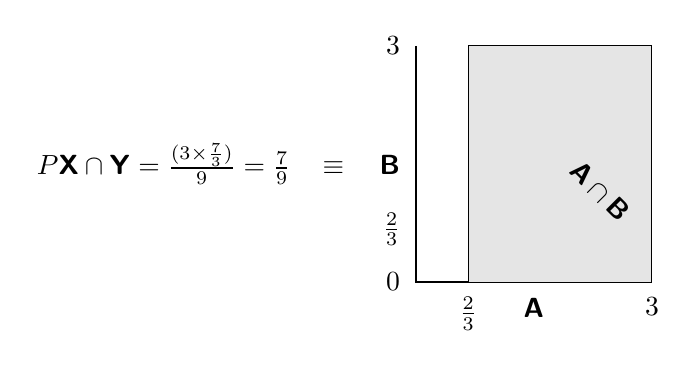
\begin{tikzpicture}
\draw[thick] (0,3) node[left=2pt] {$3$} -- node[left=2pt] {$\Prob{\Event{X}\cap\Event{Y}} = \frac{(3\times\frac{7}{3})}{9} = \frac{7}{9}\EquivGrid
\Event{B}$} (0,0)
 node[left=2pt] {$0$} -- node[below=2pt] {$\Event{A}$} (3,0) node[below=2pt] {$3$};
\draw[line width=0mm,fill=gray!20] (3,0) -- (3,3) -- (0.667,3) -- (0.667,0);
\node[left=0pt,rotate=315] at (2.75, 0.75) {$\Event{A} \cap \Event{B}$};
\node[left=2pt] at (0,0.667) {$\frac{2}{3}$};
\node[below=2pt] at (0.667,0) {$\frac{2}{3}$};
 \end{tikzpicture}
\begin{align*}
\ProbGiven{\Event{X}}{\Event{Y}} &= \frac{\Prob{\Event{X}\cap\Event{Y}}}{\Prob{\Event{Y}}}\\
&= \frac{\Prob{\Event{Y}}}{\Prob{\Event{Y}}}\\
&= 1\\
\end{align*}


\SubProblem{Find the probability \ProbGiven{\Event{Y}}{\Event{X}}.}
\begin{align*}
\ProbGiven{\Event{Y}}{\Event{X}} &= \frac{\Prob{\Event{X}\cap\Event{Y}}}{\Prob{\Event{X}}}\\
&= \frac{\frac{7}{9}}{\frac{77}{81}}\\
&= \frac{\frac{63}{81}}{\frac{77}{81}}\\
&= \frac{63}{77}\\
&= \frac{9}{11} \approx 0.\overline{81}\\
\end{align*}


\SubProblem{Find the probability \Prob{\Event{W} \cap \Event{Y}}.}
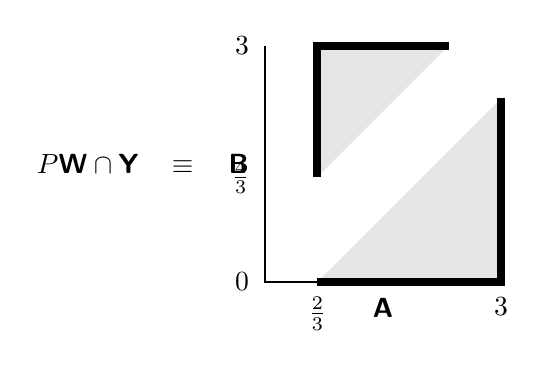
\begin{tikzpicture}
\draw[thick] (0,3) node[left=2pt] {$3$} -- node[left=2pt] {$\Prob{\Event{W}\cap\Event{Y}}\EquivGrid
\Event{B}$} (0,0)
 node[left=2pt] {$0$} -- node[below=2pt] {$\Event{A}$} (3,0) node[below=2pt] {$3$};
\draw[line width=1mm,fill=gray!20] (0.667,1.333) -- (0.667,3) -- (2.333,3);
\draw[line width=1mm,fill=gray!20] (0.667,0) -- (3,0) -- (3,2.333);
\node[left=2pt] at (0,1.333) {$\frac{4}{3}$};
\node[below=2pt] at (0.667,0) {$\frac{2}{3}$};
\end{tikzpicture}
\begin{align*}
\Prob{\Event{W}\cap\Event{Y}} &= \frac{\frac{1}{2}\times(\frac{5}{3})^2 + \frac{1}{2}\times(\frac{7}{3})^2}{(\frac{9}{3})^2}\\
&= \frac{\frac{1}{2}\times\frac{25}{9} + \frac{1}{2}\times\frac{49}{9}}{\frac{81}{9}}\\
&= \frac{\frac{25}{18} + \frac{49}{18}}{\frac{81}{9}}\\
&= \frac{\frac{74}{18}}{\frac{81}{9}}\\
&= \frac{\frac{37}{9}}{\frac{81}{9}}\\
&= \frac{37}{81} \approx 0.4568\\
\end{align*}


\SubProblem{Find the probability \ProbGiven{\Event{X}}{\Event{W}}.}
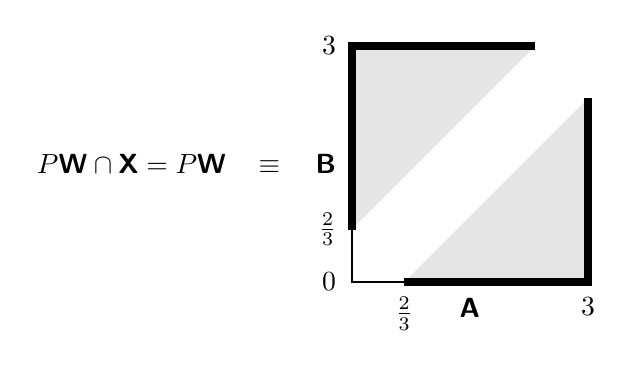
\begin{tikzpicture}
\draw[thick] (0,3) node[left=2pt] {$3$} -- node[left=2pt] {$\Prob{\Event{W}\cap\Event{X}} = \Prob{\Event{W}}\EquivGrid
\Event{B}$} (0,0)
 node[left=2pt] {$0$} -- node[below=2pt] {$\Event{A}$} (3,0) node[below=2pt] {$3$};
\draw[line width=1mm,fill=gray!20] (0,0.667) -- (0,3) -- (2.333,3);
\draw[line width=1mm,fill=gray!20] (0.667,0) -- (3,0) -- (3,2.333);
\node[left=2pt] at (0,0.667) {$\frac{2}{3}$};
\node[below=2pt] at (0.667,0) {$\frac{2}{3}$};
\end{tikzpicture}
\begin{align*}
\Prob{\Event{W}\cap\Event{X}} &= \frac{\Prob{\Event{W}\cap\Event{X}}}{\Prob{\Event{W}}}\\
&= \frac{\Prob{\Event{W}}}{\Prob{\Event{W}}}\\
&= \frac{\frac{7}{9}}{\frac{7}{9}}\\
&= 1\\
\end{align*}

If \Event{W} occurs then \Event{X} must occur!



\SubProblem{Find the probability \ProbGiven{\Event{X}}{\Event{Z}}.}

Since $\Prob{\Event{Z}} = 0$, this means that \Event{Z} is impossible.
Additionally, $\Event{X}\cap\Event{Z} \not = \emptyset$ as there is a line from $\Parens{\frac{2}{3},\,\frac{2}{3}}$ to $\Parens{3,\,3}$.
Hence, $\Event{X}$ is not independent from $\Event{Z}$. 
Because of these facts, we arrive at an unfortunate situation.
We cannot reason about \ProbGiven{\Event{X}}{\Event{Z}}, because we have the fact $\Prob{\Event{Z}} = 0$ this makes the problem statement equivalent to asking ``if we are given that the impossible occurs then what is the probability \Event{X} occurs?''

Therefore, \ProbGiven{\Event{X}}{\Event{Z}} is unknowable.



\Problem{%
You have two fair \emph{four-sided} dice, one green and one blue, called \Die{1} \& \Die{2}, respectively.\\[5mm]
$\hspace*{8mm}\Die{1} \text{ has outcomes } \Omega_{\Die{1}} = \{\,\NumA{1},\,\NumA{2},\,\NumA{3},\,\NumA{4}\,\}$.\\
$\hspace*{8mm}\Die{2} \text{ has outcomes } \Omega_{\Die{2}} = \{\,\NumB{1},\,\NumB{2},\,\NumB{3},\,\NumB{4}\,\}$.\\[5mm]
Each dice roll is independent of all others, and all faces are equally likely to come out on top when the dice is rolled.
Suppose you roll the dice twice.
Consider the following events:\\[5mm]
\BulletLine{A}
{The total of two dice is \Num{8}.}
{\RandVar{\Die{1}} + \RandVar{\Die{2}} = \Num{8}}
\BulletLine{B}
{At least one die resulted in \Num{4}.}
{\RandVar{\Die{1}} = \NumA{4}\;\lor\;\RandVar{\Die{2}} = \NumB{4}}
\BulletLine{C}
{At least one die resulted in \Num{1}.}
{\RandVar{\Die{1}} = \NumA{1}\;\lor\;\RandVar{\Die{2}} = \NumB{1}}
\BulletLine{D}
{The total of two dice is \Num{5}.}
{\RandVar{\Die{1}} + \RandVar{\Die{2}} = \Num{5}}
\BulletLine{E}
{The difference between the dice is exactly \Num{1}.}
{\left|\RandVar{\Die{1}} - \RandVar{\Die{2}}\right| = \Num{1}}
\BulletLine{F}
{The green die is less than the blue die.}
{\RandVar{\Die{1}} < \RandVar{\Die{2}}}
\Hint{Draw a $4 \times 4$ grid enumerating the all possible rolls of the dice.}%
}

\newcommand{\Bc}{\cellcolor{blue!20}}

\[
\Prob{\Event{A}} = \frac{1}{16} \EquivGrid
\begin{NiceArray}{*{5}{c}}[hvlines] 
\diagbox{\Die{1}}{\Die{2}} & \NumA{1} & \NumA{2} & \NumA{3} & \NumA{4}\\
~~~~\NumB{1}~~~~ & \Parens{\NumA{1},\NumB{1}} & \Parens{\NumA{2},\NumB{1}} & \Parens{\NumA{3},\NumB{1}} & \Parens{\NumA{4},\NumB{1}} \\
\NumB{2} & \Parens{\NumA{1},\NumB{2}} & \Parens{\NumA{2},\NumB{2}} & \Parens{\NumA{3},\NumB{2}} & \Parens{\NumA{4},\NumB{2}} \\
\NumB{3} & \Parens{\NumA{1},\NumB{3}} & \Parens{\NumA{2},\NumB{3}} & \Parens{\NumA{3},\NumB{3}} & \Parens{\NumA{4},\NumB{3}} \\
\NumB{4} & \Parens{\NumA{1},\NumB{4}} & \Parens{\NumA{2},\NumB{4}} & \Parens{\NumA{3},\NumB{4}} & \Bc\Parens{\NumA{4},\NumB{4}} \\
\end{NiceArray}
\]

\[
\Prob{\Event{B}} = \frac{7}{16} \EquivGrid
\begin{NiceArray}{*{5}{c}}[hvlines] 
\diagbox{\Die{1}}{\Die{2}} & \NumA{1} & \NumA{2} & \NumA{3} & \NumA{4}\\
~~~~\NumB{1}~~~~ & \Parens{\NumA{1},\NumB{1}} & \Parens{\NumA{2},\NumB{1}} & \Parens{\NumA{3},\NumB{1}} & \Bc\Parens{\NumA{4},\NumB{1}} \\
\NumB{2} & \Parens{\NumA{1},\NumB{2}} & \Parens{\NumA{2},\NumB{2}} & \Parens{\NumA{3},\NumB{2}} & \Bc\Parens{\NumA{4},\NumB{2}} \\
\NumB{3} & \Parens{\NumA{1},\NumB{3}} & \Parens{\NumA{2},\NumB{3}} & \Parens{\NumA{3},\NumB{3}} & \Bc\Parens{\NumA{4},\NumB{3}} \\
\NumB{4} & \Bc\Parens{\NumA{1},\NumB{4}} & \Bc\Parens{\NumA{2},\NumB{4}} & \Bc\Parens{\NumA{3},\NumB{4}} & \Bc\Parens{\NumA{4},\NumB{4}} \\
\end{NiceArray}
\]

\[
\Prob{\Event{C}} = \frac{7}{16} \EquivGrid
\begin{NiceArray}{*{5}{c}}[hvlines] 
\diagbox{\Die{1}}{\Die{2}} & \NumA{1} & \NumA{2} & \NumA{3} & \NumA{4}\\
~~~~\NumB{1}~~~~ & \Bc\Parens{\NumA{1},\NumB{1}} & \Bc\Parens{\NumA{2},\NumB{1}} & \Bc\Parens{\NumA{3},\NumB{1}} & \Bc\Parens{\NumA{4},\NumB{1}} \\
\NumB{2} & \Bc\Parens{\NumA{1},\NumB{2}} & \Parens{\NumA{2},\NumB{2}} & \Parens{\NumA{3},\NumB{2}} & \Parens{\NumA{4},\NumB{2}} \\
\NumB{3} & \Bc\Parens{\NumA{1},\NumB{3}} & \Parens{\NumA{2},\NumB{3}} & \Parens{\NumA{3},\NumB{3}} & \Parens{\NumA{4},\NumB{3}} \\
\NumB{4} & \Bc\Parens{\NumA{1},\NumB{4}} & \Parens{\NumA{2},\NumB{4}} & \Parens{\NumA{3},\NumB{4}} & \Parens{\NumA{4},\NumB{4}} \\
\end{NiceArray}
\]

\[
\Prob{\Event{D}} = \frac{4}{16} \EquivGrid
\begin{NiceArray}{*{5}{c}}[hvlines] 
\diagbox{\Die{1}}{\Die{2}} & \NumA{1} & \NumA{2} & \NumA{3} & \NumA{4}\\
~~~~\NumB{1}~~~~ & \Parens{\NumA{1},\NumB{1}} & \Parens{\NumA{2},\NumB{1}} & \Parens{\NumA{3},\NumB{1}} & \Bc\Parens{\NumA{4},\NumB{1}} \\
\NumB{2} & \Parens{\NumA{1},\NumB{2}} & \Parens{\NumA{2},\NumB{2}} & \Bc\Parens{\NumA{3},\NumB{2}} & \Parens{\NumA{4},\NumB{2}} \\
\NumB{3} & \Parens{\NumA{1},\NumB{3}} & \Bc\Parens{\NumA{2},\NumB{3}} & \Parens{\NumA{3},\NumB{3}} & \Parens{\NumA{4},\NumB{3}} \\
\NumB{4} & \Bc\Parens{\NumA{1},\NumB{4}} & \Parens{\NumA{2},\NumB{4}} & \Parens{\NumA{3},\NumB{4}} & \Parens{\NumA{4},\NumB{4}} \\
\end{NiceArray}
\]

\[
\Prob{\Event{E}} = \frac{6}{16} \EquivGrid
\begin{NiceArray}{*{5}{c}}[hvlines] 
\diagbox{\Die{1}}{\Die{2}} & \NumA{1} & \NumA{2} & \NumA{3} & \NumA{4}\\
~~~~\NumB{1}~~~~ & \Parens{\NumA{1},\NumB{1}} & \Bc\Parens{\NumA{2},\NumB{1}} & \Parens{\NumA{3},\NumB{1}} & \Parens{\NumA{4},\NumB{1}} \\
\NumB{2} & \Bc\Parens{\NumA{1},\NumB{2}} & \Parens{\NumA{2},\NumB{2}} & \Bc\Parens{\NumA{3},\NumB{2}} & \Parens{\NumA{4},\NumB{2}} \\
\NumB{3} & \Parens{\NumA{1},\NumB{3}} & \Bc\Parens{\NumA{2},\NumB{3}} & \Parens{\NumA{3},\NumB{3}} & \Bc\Parens{\NumA{4},\NumB{3}} \\
\NumB{4} & \Parens{\NumA{1},\NumB{4}} & \Parens{\NumA{2},\NumB{4}} & \Bc\Parens{\NumA{3},\NumB{4}} & \Parens{\NumA{4},\NumB{4}} \\
\end{NiceArray}
\]

\[
\Prob{\Event{F}} = \frac{6}{16} \EquivGrid
\begin{NiceArray}{*{5}{c}}[hvlines] 
\diagbox{\Die{1}}{\Die{2}} & \NumA{1} & \NumA{2} & \NumA{3} & \NumA{4}\\
~~~~\NumB{1}~~~~ & \Parens{\NumA{1},\NumB{1}} & \Parens{\NumA{2},\NumB{1}} & \Parens{\NumA{3},\NumB{1}} & \Parens{\NumA{4},\NumB{1}} \\
\NumB{2} & \Bc\Parens{\NumA{1},\NumB{2}} & \Parens{\NumA{2},\NumB{2}} & \Parens{\NumA{3},\NumB{2}} & \Parens{\NumA{4},\NumB{2}} \\
\NumB{3} & \Bc\Parens{\NumA{1},\NumB{3}} & \Bc\Parens{\NumA{2},\NumB{3}} & \Parens{\NumA{3},\NumB{3}} & \Parens{\NumA{4},\NumB{3}} \\
\NumB{4} & \Bc\Parens{\NumA{1},\NumB{4}} & \Bc\Parens{\NumA{2},\NumB{4}} & \Bc\Parens{\NumA{3},\NumB{4}} & \Parens{\NumA{4},\NumB{4}} \\
\end{NiceArray}
\]

\SubProblem{Is event \Event{A} independent of event \Event{B}?}
\[
\Prob{\Event{A} \cap \Event{B}} = \frac{1}{16} \EquivGrid
\begin{NiceArray}{*{5}{c}}[hvlines] 
\diagbox{\Die{1}}{\Die{2}} & \NumA{1} & \NumA{2} & \NumA{3} & \NumA{4}\\
~~~~\NumB{1}~~~~ & \Parens{\NumA{1},\NumB{1}} & \Parens{\NumA{2},\NumB{1}} & \Parens{\NumA{3},\NumB{1}} & \Parens{\NumA{4},\NumB{1}} \\
\NumB{2} & \Parens{\NumA{1},\NumB{2}} & \Parens{\NumA{2},\NumB{2}} & \Parens{\NumA{3},\NumB{2}} & \Parens{\NumA{4},\NumB{2}} \\
\NumB{3} & \Parens{\NumA{1},\NumB{3}} & \Parens{\NumA{2},\NumB{3}} & \Parens{\NumA{3},\NumB{3}} & \Parens{\NumA{4},\NumB{3}} \\
\NumB{4} & \Parens{\NumA{1},\NumB{4}} & \Parens{\NumA{2},\NumB{4}} & \Parens{\NumA{3},\NumB{4}} & \Bc\Parens{\NumA{4},\NumB{4}} \\
\end{NiceArray}
\]
\begin{align*}
\ProbGiven{\Event{A}}{\Event{B}} &=  \frac{\Prob{\Event{A} \cap \Event{B}}}{\Prob{\Event{B}}}\\
&= \frac{\frac{1}{16}}{\frac{7}{16}}\\
&= \frac{1}{7}\\
\end{align*}
\[
\Prob{A} = \frac{1}{16} \not = \frac{7}{16} = \ProbGiven{\Event{A}}{\Event{B}} \implies \text{\Event{A} \emph{is not} independent of event \Event{B}}
\]


\SubProblem{Is event \Event{A} independent of event \Event{C}?}
\begin{align*}
\ProbGiven{\Event{A}}{\Event{C}} &=  \frac{\Prob{\Event{A} \cap \Event{C}}}{\Prob{\Event{C}}}\\
&= \frac{\frac{0}{16}}{\frac{7}{16}}\qquad\textbf{because~}\Event{A} \cap \Event{C} = \emptyset \implies \Prob{\Event{A} \cap \Event{C}} = 0\\ 
&= \frac{0}{7}\\
&= 0\\
\end{align*}
\[
\Prob{A} = \frac{1}{16} \not = \frac{0}{16} = \ProbGiven{\Event{A}}{\Event{C}} \implies \text{\Event{A} \emph{is not} independent of event \Event{C}}
\]


\SubProblem{Are events \Event{E} and \Event{F} independent?}
\[
\Prob{\Event{E} \cap \Event{F}} = \frac{3}{16} \EquivGrid
\begin{NiceArray}{*{5}{c}}[hvlines] 
\diagbox{\Die{1}}{\Die{2}} & \NumA{1} & \NumA{2} & \NumA{3} & \NumA{4}\\
~~~~\NumB{1}~~~~ & \Parens{\NumA{1},\NumB{1}} & \Parens{\NumA{2},\NumB{1}} & \Parens{\NumA{3},\NumB{1}} & \Parens{\NumA{4},\NumB{1}} \\
\NumB{2} & \Bc\Parens{\NumA{1},\NumB{2}} & \Parens{\NumA{2},\NumB{2}} & \Parens{\NumA{3},\NumB{2}} & \Parens{\NumA{4},\NumB{2}} \\
\NumB{3} & \Parens{\NumA{1},\NumB{3}} & \Bc\Parens{\NumA{2},\NumB{3}} & \Parens{\NumA{3},\NumB{3}} & \Parens{\NumA{4},\NumB{3}} \\
\NumB{4} & \Parens{\NumA{1},\NumB{4}} & \Parens{\NumA{2},\NumB{4}} & \Bc\Parens{\NumA{3},\NumB{4}} & \Parens{\NumA{4},\NumB{4}} \\
\end{NiceArray}
\]
\begin{minipage}[t]{.49\textwidth}
\begin{align*}
\ProbGiven{\Event{E}}{\Event{F}} &=  \frac{\Prob{\Event{E} \cap \Event{F}}}{\Prob{\Event{F}}}\\
&= \frac{\frac{3}{16}}{\frac{6}{16}}\\
&= \frac{3}{6}\\
&= \frac{1}{2}\\
\end{align*}
\end{minipage}
\begin{minipage}[t]{.49\textwidth}
\begin{align*}
\ProbGiven{\Event{F}}{\Event{E}} &=  \frac{\Prob{\Event{E} \cap \Event{F}}}{\Prob{\Event{E}}}\\
&= \frac{\frac{3}{16}}{\frac{6}{16}}\\
&= \frac{3}{6}\\
&= \frac{1}{2}\\
\end{align*}
\end{minipage}
\[
\Prob{E} = \frac{6}{16} \not = \frac{1}{2} = \ProbGiven{\Event{E}}{\Event{F}} \implies \text{\Event{E} \emph{is not} independent of event \Event{F}}
\]
\[
\Prob{F} = \frac{6}{16} \not = \frac{1}{2} = \ProbGiven{\Event{F}}{\Event{E}} \implies \text{\Event{F} \emph{is not} independent of event \Event{E}}
\]


\SubProblem{Are events \Event{E} and \Event{F} independent given event D?}
\[
\phantom{\Event{E}\cap\;}\Prob{\Event{D} \cap \Event{F}} = \frac{2}{16} \EquivGrid
\begin{NiceArray}{*{5}{c}}[hvlines] 
\diagbox{\Die{1}}{\Die{2}} & \NumA{1} & \NumA{2} & \NumA{3} & \NumA{4}\\
~~~~\NumB{1}~~~~ & \Parens{\NumA{1},\NumB{1}} & \Parens{\NumA{2},\NumB{1}} & \Parens{\NumA{3},\NumB{1}} & \Parens{\NumA{4},\NumB{1}} \\
\NumB{2} & \Parens{\NumA{1},\NumB{2}} & \Parens{\NumA{2},\NumB{2}} & \Parens{\NumA{3},\NumB{2}} & \Parens{\NumA{4},\NumB{2}} \\
\NumB{3} & \Parens{\NumA{1},\NumB{3}} & \Bc\Parens{\NumA{2},\NumB{3}} & \Parens{\NumA{3},\NumB{3}} & \Parens{\NumA{4},\NumB{3}} \\
\NumB{4} & \Bc\Parens{\NumA{1},\NumB{4}} & \Parens{\NumA{2},\NumB{4}} & \Parens{\NumA{3},\NumB{4}} & \Parens{\NumA{4},\NumB{4}} \\
\end{NiceArray}
\]
\[
\phantom{\Event{E}\cap\;}\Prob{\Event{D} \cap \Event{E}} = \frac{2}{16} \EquivGrid
\begin{NiceArray}{*{5}{c}}[hvlines] 
\diagbox{\Die{1}}{\Die{2}} & \NumA{1} & \NumA{2} & \NumA{3} & \NumA{4}\\
~~~~\NumB{1}~~~~ & \Parens{\NumA{1},\NumB{1}} & \Parens{\NumA{2},\NumB{1}} & \Parens{\NumA{3},\NumB{1}} & \Parens{\NumA{4},\NumB{1}} \\
\NumB{2} & \Parens{\NumA{1},\NumB{2}} & \Parens{\NumA{2},\NumB{2}} & \Bc\Parens{\NumA{3},\NumB{2}} & \Parens{\NumA{4},\NumB{2}} \\
\NumB{3} & \Parens{\NumA{1},\NumB{3}} & \Bc\Parens{\NumA{2},\NumB{3}} & \Parens{\NumA{3},\NumB{3}} & \Parens{\NumA{4},\NumB{3}} \\
\NumB{4} & \Parens{\NumA{1},\NumB{4}} & \Parens{\NumA{2},\NumB{4}} & \Parens{\NumA{3},\NumB{4}} & \Parens{\NumA{4},\NumB{4}} \\
\end{NiceArray}
\]
\[
\Prob{\Event{D}\cap\Event{E}\cap\Event{F}} = \frac{1}{16} \EquivGrid
\begin{NiceArray}{*{5}{c}}[hvlines] 
\diagbox{\Die{1}}{\Die{2}} & \NumA{1} & \NumA{2} & \NumA{3} & \NumA{4}\\
~~~~\NumB{1}~~~~ & \Parens{\NumA{1},\NumB{1}} & \Parens{\NumA{2},\NumB{1}} & \Parens{\NumA{3},\NumB{1}} & \Parens{\NumA{4},\NumB{1}} \\
\NumB{2} & \Parens{\NumA{1},\NumB{2}} & \Parens{\NumA{2},\NumB{2}} & \Parens{\NumA{3},\NumB{2}} & \Parens{\NumA{4},\NumB{2}} \\
\NumB{3} & \Parens{\NumA{1},\NumB{3}} & \Bc\Parens{\NumA{2},\NumB{3}} & \Parens{\NumA{3},\NumB{3}} & \Parens{\NumA{4},\NumB{3}} \\
\NumB{4} & \Parens{\NumA{1},\NumB{4}} & \Parens{\NumA{2},\NumB{4}} & \Parens{\NumA{3},\NumB{4}} & \Parens{\NumA{4},\NumB{4}} \\
\end{NiceArray}
\]
\begin{align*}
\ProbGiven{\Event{E}}{\Event{F}\cap\Event{D}} &=\\
\frac{\Prob{\Event{E} \cap \Parens{\Event{F}\cap\Event{D}}}}{\Prob{\Event{F}\cap\Event{D}}} &=\\
\frac{\frac{1}{16}}{\frac{2}{16}} &=\\
\frac{1}{2} &= \frac{1}{2}\\
&= \frac{2}{4}\\
&=  \frac{\frac{2}{16}}{\frac{4}{16}}\\
&=  \frac{\Prob{\Event{E}\cap\Event{D}}}{\Prob{\Event{D}}}\\
&= \ProbGiven{\Event{E}}{\Event{D}} \\
\end{align*}
\[
\ProbGiven{\Event{E}}{\Event{F}\cap\Event{D}} = \frac{1}{2} = \ProbGiven{\Event{E}}{\Event{D}} \implies \text{\Event{E} given \Event{D} \textbf{is} independent of \Event{F} given \Event{D}}
\]

\begin{align*}
\ProbGiven{\Event{F}}{\Event{E}\cap\Event{D}} &=\\
\frac{\Prob{\Event{F} \cap \Parens{\Event{E}\cap\Event{D}}}}{\Prob{\Event{E}\cap\Event{D}}} &=\\
\frac{\frac{1}{16}}{\frac{2}{16}} &=\\
\frac{1}{2} &=  \frac{1}{2}\\
&=  \frac{\frac{2}{16}}{\frac{4}{16}}\\
&=  \frac{\Prob{\Event{F}\cap\Event{D}}}{\Prob{\Event{D}}}\\
&= \ProbGiven{\Event{F}}{\Event{D}} \\
\end{align*}

\[
\ProbGiven{\Event{F}}{\Event{E}\cap\Event{D}} = \frac{1}{2} = \ProbGiven{\Event{F}}{\Event{D}} \implies \text{\Event{F} given \Event{D} \textbf{is} independent of \Event{E} given \Event{D}}
\]

\newcommand{\Coin}[1]{\ensuremath{\mathcal{C}_{\mathbf{#1}}}}

\Problem{
Consider three coins, \Coin{1}, \Coin{2}, and \Coin{3}.
Coins \Coin{1} and \Coin{2} are fair coins:
$$\ProbGiven{\Heads}{\Coin{1}} = \frac{1}{2} = \ProbGiven{\Heads}{\Coin{2}}$$
However, coin \Coin{3} is biased, yielding heads with the probability: 
$$\ProbGiven{\Heads}{\Coin{3}} =  \frac{3}{4}$$\\
You select uniformly at random one of  \Coin{1}, \Coin{2}, or \Coin{3}, and then toss the selected coin 3 times, yielding the outcome \SetNote{\Heads,\,\Heads,\,\Heads}.\\[5mm]
\textit{What is the probability you selected the biased coin \Coin{3}?}
}
\begin{minipage}[t]{.49\textwidth}
\begin{align*}
\Prob{\Heads,\,\Heads,\,\Heads} &= \frac{1 \times \ProbGiven{\Heads}{\Coin{3}}^3 + 2 \times (\ProbGiven{\Heads}{\Coin{1}})^3}{3}\\
&= \frac{1 \times (\frac{3}{4})^3 + 2 \times (\frac{1}{2})^3}{3}\\
&= \frac{\frac{27}{64} + 2 \times \frac{1}{8}}{3}\\
&= \frac{\frac{27}{64} + \frac{2}{8}}{3}\\
&= \frac{\frac{27}{64} + \frac{16}{64}}{3}\\
&= \frac{\frac{43}{64}}{3}\\
&= \frac{43}{192}\\
\end{align*}
\end{minipage}
\begin{minipage}[t]{.49\textwidth}
\begin{align*}
\ProbGiven{\Heads,\,\Heads,\,\Heads}{\Coin{3}} &= \ProbGiven{\Heads}{\Coin{3}}^3\\
&= \Parens{\frac{3}{4}}^3\\
&= \frac{27}{64}
\end{align*}
\end{minipage}


\begin{align*}
\ProbGiven{\Coin{3}}{\Heads,\,\Heads,\,\Heads} &= \frac{\ProbGiven{\Heads,\,\Heads,\,\Heads}{\Coin{3}} \times \Prob{\Coin{3}} }{\Prob{\Heads,\,\Heads,\,\Heads}}\\
&= \frac{\frac{27}{64} \times \frac{1}{3}}{\frac{43}{192}}\\
&= \frac{\frac{27}{192}}{\frac{43}{192}}\\
&= \frac{27}{43} \approx 0.628
\end{align*}



\StartExtraCredit
\Problem{%
Which is the most preferable from these mutually exclusive options?\\[5mm]%
\setstretch{1.7}
\hspace*{1cm}$\tabbedLongunderstack[l]{
\,\heartsuit\,\quad\text{Pursue your passion}\\
\;\$\:\quad\text{Take the money}%
}$%
}


\end{document}
